% =============================================================================
% main.tex — Rapid Fertility Collapse in Latin America (Draft 1)
% Overleaf-ready. Compile: pdflatex -> bibtex -> pdflatex x2.
% Build instruction: DRAFT1_build_instruction_Fina.md (Fina, 2026-07-12).
% Numbers trace to FINA_results_for_draft1_2026-07-12.md and the endorsed memos.
% =============================================================================
\documentclass[11pt]{article}
% preamble.tex — Rapid Fertility Collapse in Latin America (Draft 1)
% Minimal, portable, Overleaf-ready. No absolute paths anywhere.
\usepackage[margin=1.1in]{geometry}
\usepackage{amsmath}
\usepackage{graphicx}
\usepackage{booktabs}
\usepackage{subcaption}
\usepackage[round]{natbib}
\usepackage{siunitx}
\usepackage{csquotes}
\usepackage{algorithm}
\usepackage{algpseudocode}
\usepackage[hidelinks]{hyperref}

\graphicspath{{figures/}}

% ---- notation macros (model section + ODD appendix) ----
\newcommand{\kb}{\kappa(b)}          % cohort marriage-entry multiplier
\newcommand{\phib}{\varphi(b)}       % cohort formation tilt
\newcommand{\pit}{\pi(t)}            % exogenous period shifter (robustness spec)
\newcommand{\Sng}{\mathsf{S}}        % single
\newcommand{\Coh}{\mathsf{C}}        % cohabiting
\newcommand{\Mar}{\mathsf{M}}        % married

% ---- editorial ----
\newcommand{\todo}[1]{\textbf{[TODO: #1]}}


\title{Cohort Replacement, Not Cascade:\\
Union Composition and the Rapid Fertility Collapse in Latin America\thanks{%
Draft 2 (2026-07-12), not for circulation. Prepared within the Demographic Fiscal
Dynamics (DFD) project. Replication code, figure data, and the ODD protocol are
described in Appendix~\ref{app:odd}; all series carry per-row source and methodology
flags in the project repository.}}
\author{H\'ector Juan Villarreal P\'aez\\
\small Tecnol\'ogico de Monterrey, School of Social Sciences and Government
% \and (coauthors TBD)
}
\date{July 2026 --- Draft 2}

\begin{document}
\maketitle

\begin{abstract}
\noindent
Several Latin American countries have experienced one of the fastest peacetime
fertility declines on record: national vital registries show total fertility falling
to near 1.1 in Costa Rica, Colombia, and Chile by 2024, while smoothed international
series largely erase the acceleration. We document this collapse against registry and
microdata sources, and locate its proximate driver in union \emph{composition}: total
union prevalence is roughly flat while marriage collapses and cohabitation substitutes.
We then discriminate between candidate mechanisms with a pre-registered,
outcome-robust design. Age--period--cohort curvature and the sign of state dependence
in pseudo-cohort panels reject a within-cohort reflexive cascade in both Costa Rica
and Colombia --- the state-dependence coefficient is positive (stabilizing) in every
specification --- and identify cohort replacement as the dominant structure, with a
small exogenous period component in Colombia. A deliberately transparent
cohort microsimulation with \emph{four} interpretable parameters --- a three-parameter
logistic decline in cohort marriage propensity and a one-parameter formation tilt,
with no social feedback --- is then shown to be \emph{sufficient} for the observed
composition collapse: it reproduces its magnitude and late-loading, and its calibrated
cohort inflection point (birth cohorts 1989--1992) independently recovers the
age--period--cohort crossover it was never fit to. We interpret the findings as
channel-assisted compression of the Second Demographic Transition, and state a
falsifiable out-of-sample prediction for marriage-dominant regimes.
\end{abstract}

\vspace{0.5em}
\noindent\textbf{Keywords:} fertility decline; union composition; cohabitation;
Second Demographic Transition; agent-based modeling; Latin America.

% =============================================================================
% §1 Introduction — phenomenon (R1); puzzle; contributions C1–C5; the arc;
% the roadmap / division-of-labor paragraph (Fina §3, mandate A).
% =============================================================================
\section{Introduction}
\label{sec:intro}

Between 2015 and 2024, several Latin American countries experienced fertility
declines of a speed with few peacetime precedents. Costa Rica's total fertility
rate (TFR) fell from 1.83 in 2010 to 1.12 in 2024 --- a 39 percent decline, most
of it after 2016. Colombia's national registry series fell from 1.7 to 1.1 in
under a decade; Chile reached 1.03 in 2024. These are not marginal adjustments
within a below-replacement regime; they are collapses to among the lowest
fertility levels ever recorded, in middle-income countries, within roughly
eight years --- the kind of tempo that has moved global demographic
projection debates from convergence scenarios to genuine uncertainty about
the fertility floor \citep{fernandezvillaverde2026}. Remarkably, the acceleration is barely visible in the smoothed
international series most analysts consult: World Bank and World Population
Prospects figures, which interpolate through model schedules, trail the national
registries by up to half a child per woman at the end of the sample
(Section~\ref{sec:phenomenon}).

The speed is the puzzle. Classical transition frameworks --- including the Second
Demographic Transition (SDT) that correctly anticipated the \emph{direction} of
change \citep{lesthaeghe1986twee, vandekaa1987, lesthaeghe2010} --- describe
ideational and institutional change diffusing across generations. They give no
mechanism for a national TFR losing a third of its level in eight years. Fast
declines invite fast-dynamics explanations, and the current literature and public
debate lean readily on \emph{reflexive} accounts: social-media-amplified norm
cascades, coordination tipping points, self-reinforcing childlessness. These
mechanisms are theoretically attractive precisely because they are fast. Whether
the data actually exhibit their signature is the question this paper answers.

We make five contributions. \textbf{First} (measurement), we document the
collapse against national vital registries and household microdata rather than
smoothed international series, showing that raw annual births fell 18--47 percent
across the collapse countries while the female population of reproductive age
grew --- the decline is behavioral, not a denominator artifact --- and that the
standard international series systematically erase its acceleration.
\textbf{Second} (state variable), we show that the proximate driver is union
\emph{composition}: total union prevalence among women 20--39 is roughly flat
while marriage collapses and cohabitation substitutes --- in Colombia, marriage
halves (20.7 to 11.9 percent) on a flat union plateau. \textbf{Third}
(identification), we discriminate between candidate mechanisms with a
pre-registered, outcome-robust design: age--period--cohort (APC) curvature
localizes the change, and the \emph{sign} of state dependence in pseudo-cohort
panels tests for reflexivity. The verdict is unambiguous: the state-dependence
coefficient is positive --- stabilizing, the opposite of a cascade signature ---
in every specification, in both countries; the structure is \emph{cohort
replacement}, with a small exogenous period component in Colombia.
\textbf{Fourth} (sufficiency), we show that a deliberately transparent cohort
microsimulation with four interpretable parameters and no social feedback is
\emph{sufficient} for the observed composition collapse --- magnitude and
late-loading --- and that its single calibrated cohort inflection point
independently recovers the APC crossover it was never fit to. \textbf{Fifth}
(interpretation), we frame the findings as \emph{channel-assisted compression}
of the SDT: change concentrates where the institutional channel --- Latin
America's long-standing consensual-union system \citep{esteve2012} --- was
already wide, which yields a falsifiable out-of-sample prediction for
marriage-dominant regimes.

The paper's arc is deliberately outcome-robust. We built the fashionable model
first: an agent-based simulation with a social-norm coordination threshold, the
formalization of the cascade narrative. The data rejected it twice --- the
calibrated threshold produced a smooth glide rather than the observed
acceleration, and the econometric cascade test returned the wrong sign in every
specification. What survived is simpler: successive cohorts arrive with lower
marriage propensity, and the stock composition follows as they flow through the
age distribution. We report the rejections as prominently as the survivor,
because the discrimination is what makes the survivor credible.

A roadmap, which is also the paper's division of labor. Registries and microdata
\emph{measure} the phenomenon (Section~\ref{sec:phenomenon}).
Section~\ref{sec:mechanisms} states the three candidate mechanisms and their
observable signatures. APC curvature and state dependence \emph{identify} the
mechanism econometrically (Section~\ref{sec:discrimination}); identification is
econometric throughout, and the simulation model is never asked to perform it.
The agent-based model \emph{tests sufficiency} of the identified mechanism ---
whether cohort replacement alone can generate what we observe --- under a
pre-registered evaluation (Section~\ref{sec:model}). The SDT \emph{frames} the
result and generates the out-of-sample prediction
(Section~\ref{sec:interpretation}). Section~\ref{sec:limitations} states the
scope conditions and data limitations; Section~\ref{sec:conclusion} concludes.

% =============================================================================
% §2 Phenomenon & measurement (M1 / R1+R2) — registry collapse; WB/WPP smoothing
% failure; union composition as state variable; data-limitations (measurement).
% =============================================================================
\section{The Phenomenon: Measurement Against Primary Sources}
\label{sec:phenomenon}

\subsection{The collapse in national vital registries}
\label{sec:registries}

Table~\ref{tab:anchors} reports the corrected national anchors. Every figure
comes from the national vital-registration system or statistical institute of
the country concerned; each series in the project repository carries per-row
source and methodology flags.

\begin{table}[t]
\centering
\caption{National TFR anchors, collapse countries and comparator. The CELADE
column reports the corresponding CELADE 2024 medium-variant estimate where a
pinned comparator exists; the systematic register--estimate gap is discussed
in the text.}
\label{tab:anchors}
\footnotesize
\begin{tabular}{@{}l l l c p{4.9cm}@{}}
\toprule
Country & Register series & Level and change & CELADE & Notes \\
\midrule
Costa Rica & INEC & $1.83 \rightarrow 1.12$ (2010--24) & 1.32 &
  register total (includes the 19.3\% of 2024 births to foreign-born mothers);
  denominator INEC-CCP post-Censo-2022, level $\pm$0.03; 2024 from INEC
  \emph{Indicadores demogr\'aficos 2024} \\
Colombia & DANE EEVV & $1.7 \rightarrow 1.1$ (2015--24) & --- &
  \emph{not} the circulating ``$2.0 \rightarrow 1.06$'', which appears in no
  DANE source \\
Chile & INE/DEIS & $1.81 \rightarrow 1.03$ (2010--24) & 1.14 &
  official TGF publication gap 2010--21 filled by births-implied TFR anchored
  to registry years \\
Argentina & DEIS/INDEC & $\approx 1.15$--$1.19$ (2024) & --- &
  no official period TGF after 2021; INDEC-anchored reconstruction, labeled
  throughout \\
Mexico (comp.) & CONAPO / ENADID & 1.89 (modeled) / 1.60 (survey, 2023) & --- &
  slow-decline comparator; the circulating ``1.55'' is not a national figure \\
\bottomrule
\end{tabular}
\end{table}

Three measurement points deserve emphasis. First, the decline is behavioral,
not a denominator artifact: in every collapse country the \emph{raw annual
birth count} fell between 18 and 47 percent while the female population aged
15--49 grew (Chile: 250{,}643 births in 2010 to 154{,}441 in 2024, $-38$
percent; Figure~\ref{fig:forensics}). No plausible revision to population
denominators reverses that.
Second, several widely circulated figures are wrong or unofficial: Colombia's
``2.0 to 1.06'' appears in no DANE source (the genuine collapse is roughly 35
percent in TFR, not 47); Argentina has published no official period TGF since
2021, so any post-2021 level is a reconstruction and should be labeled as such.
Third, the smoothed international series miss the event.
Figure~\ref{fig:smoothing} contrasts national registry series with the World
Bank/WPP series: the model-smoothed lines glide while the registries collapse,
with end-of-sample gaps up to roughly half a child per woman. The same pattern
holds for the regional projections: CELADE 2024 medium-variant estimates sit
\emph{above} the register totals by 0.20 in Costa Rica (1.32 vs.\ 1.12) and
0.11 in Chile (1.14 vs.\ 1.03) --- an optimism gap, not a register deficiency.
The Costa Rican 1.12 is the register \emph{total}: births are a near-complete
civil registry (and include the 19.3 percent of 2024 births to foreign-born
mothers --- immigrant childbearing works \emph{against} the collapse, so the
native-born decline is sharper still); the only revisable component is the
post-Censo-2022 population denominator, worth about $\pm 0.03$ on the level
and nothing on the trend. Analyses built on the international or projected
series would date the collapse late, understate its speed, and miss its
acceleration entirely.

\begin{figure}[t]
\centering
\begin{subfigure}[b]{0.48\textwidth}
  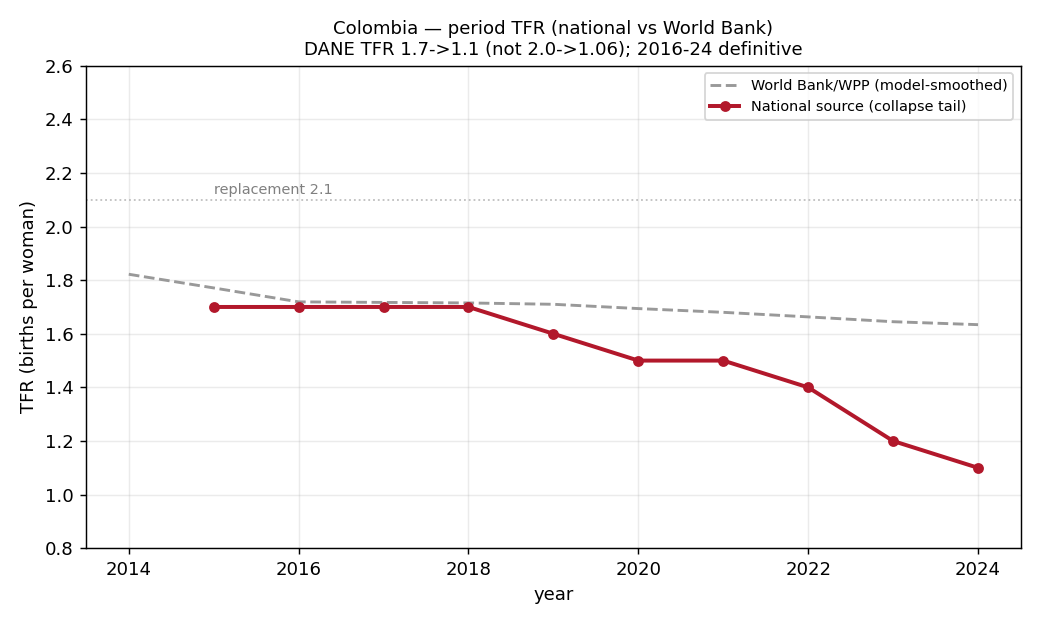
\includegraphics[width=\textwidth]{fig_tfr_registry_wb_COL.png}
  \caption{Colombia}
\end{subfigure}
\hfill
\begin{subfigure}[b]{0.48\textwidth}
  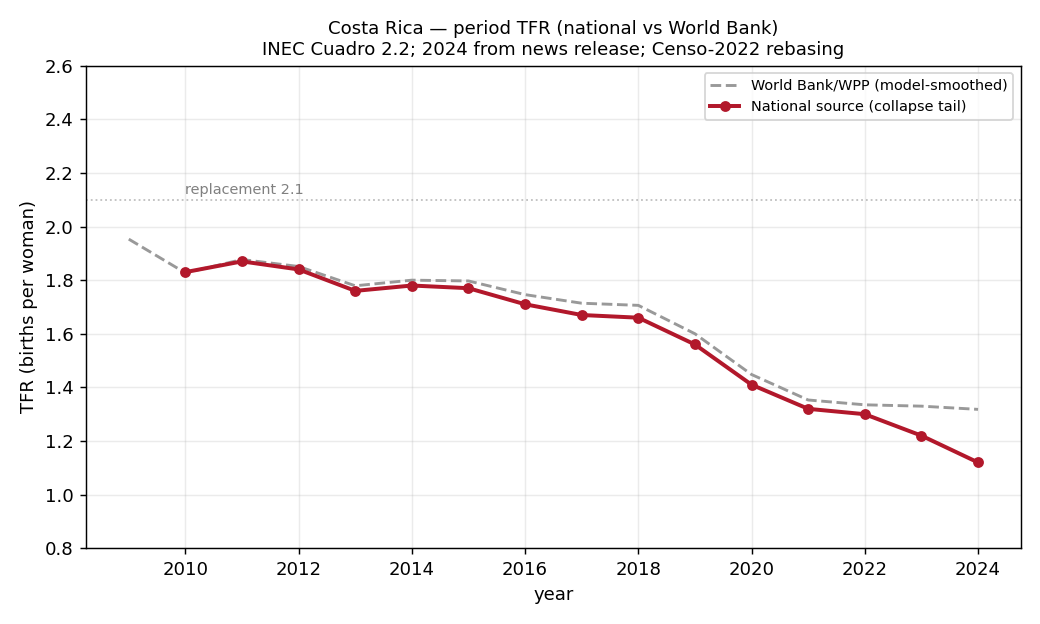
\includegraphics[width=\textwidth]{fig_tfr_registry_wb_CRI.png}
  \caption{Costa Rica}
\end{subfigure}
\caption{National registry TFR versus World Bank/WPP model-smoothed series.
The international series erase the acceleration that defines the phenomenon.}
\label{fig:smoothing}
\end{figure}

\begin{figure}[t]
\centering
\begin{subfigure}[b]{0.48\textwidth}
  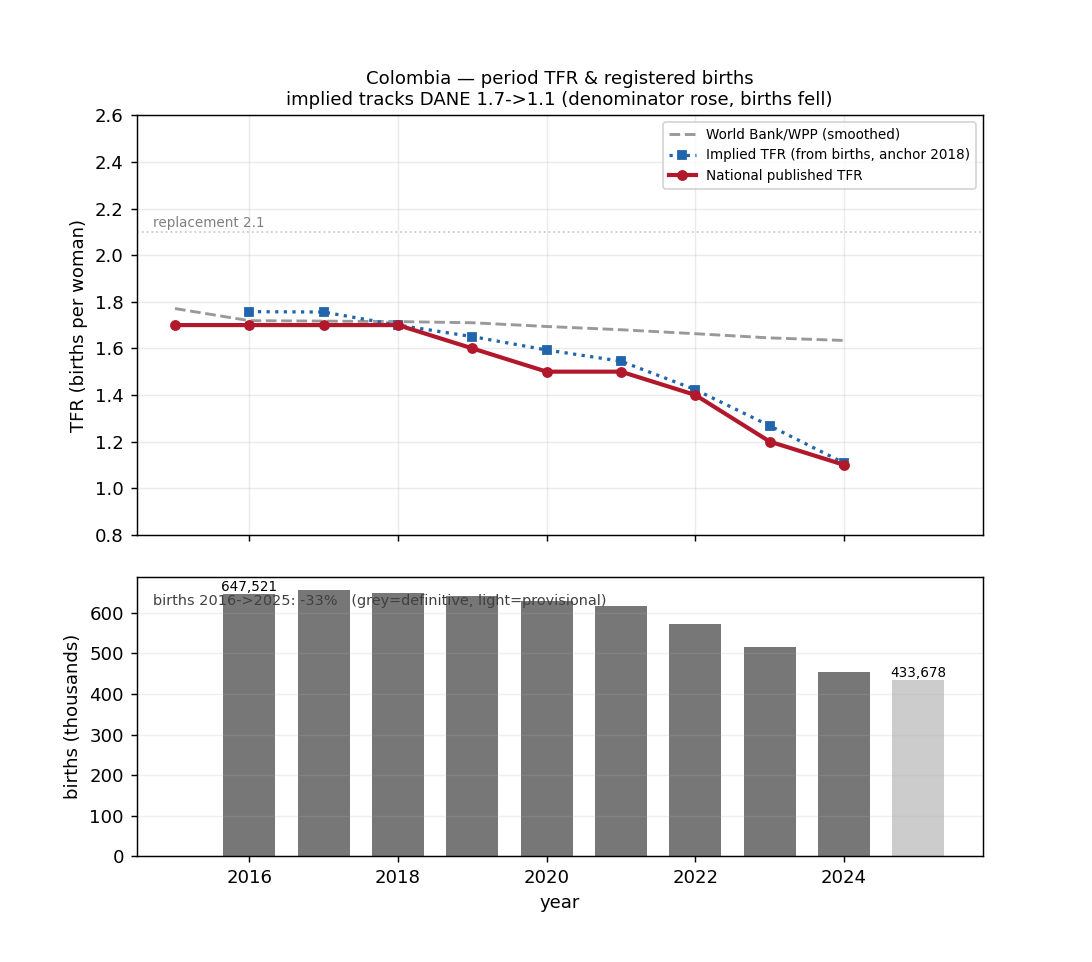
\includegraphics[width=\textwidth]{fig_forensic_panel_COL.png}
  \caption{Colombia}
\end{subfigure}
\hfill
\begin{subfigure}[b]{0.48\textwidth}
  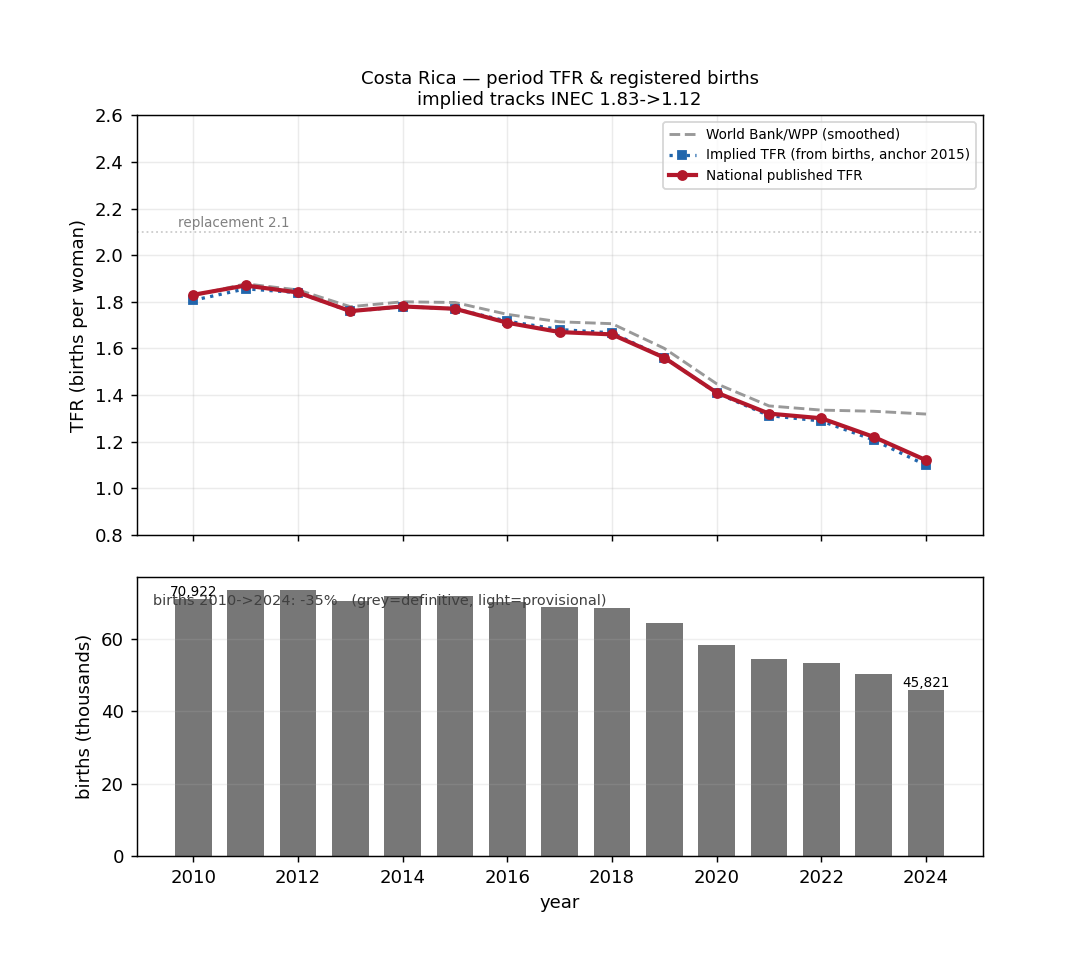
\includegraphics[width=\textwidth]{fig_forensic_panel_CRI.png}
  \caption{Costa Rica}
\end{subfigure}
\caption{Registered births and period TFR. Births-implied TFR (anchored to a
registry year) tracks the published national series: the collapse is in the
numerator, not the denominator.}
\label{fig:forensics}
\end{figure}

\subsection{The state variable: union composition}
\label{sec:composition}

What proximately drives births down? We construct annual union-composition
series for women aged 20--39, in four five-year age bands, distinguishing
\emph{married} from \emph{cohabiting} (consensual union) --- for Costa Rica from
ENAHO via INEC's REDATAM tabulations (2010--2024), and for Colombia from DANE
GEIH person-level microdata (2007--2024; eighteen annual pooled files, with the
estado-civil coding verified to be identical across the 2021--22 survey
redesign, so the downturn is not a recode).

The composition series reveal the phenomenon's structure
(Figure~\ref{fig:coupling}). In Colombia, \emph{total} union prevalence sits on
a flat plateau near 59--60 percent from 2008 to 2020 (declining moderately
thereafter), while the \emph{married} share halves --- from 20.7 to 11.9
percent --- with cohabitation substituting almost one-for-one. Costa Rica shows
the same signature: the equal-band-mean married share falls from 0.324 (2010)
to 0.166 (2024). Partnership as such is not disappearing; its \emph{composition}
is transforming, and because fertility differs across union types, composition
is the natural state variable for the fertility consequences. Throughout the
paper, the state variable is the three-way composition
$\{\Sng,\Coh,\Mar\}$ (single, cohabiting, married) --- never a binary
partnered/unpartnered.

\begin{figure}[t]
\centering
\begin{subfigure}[b]{0.48\textwidth}
  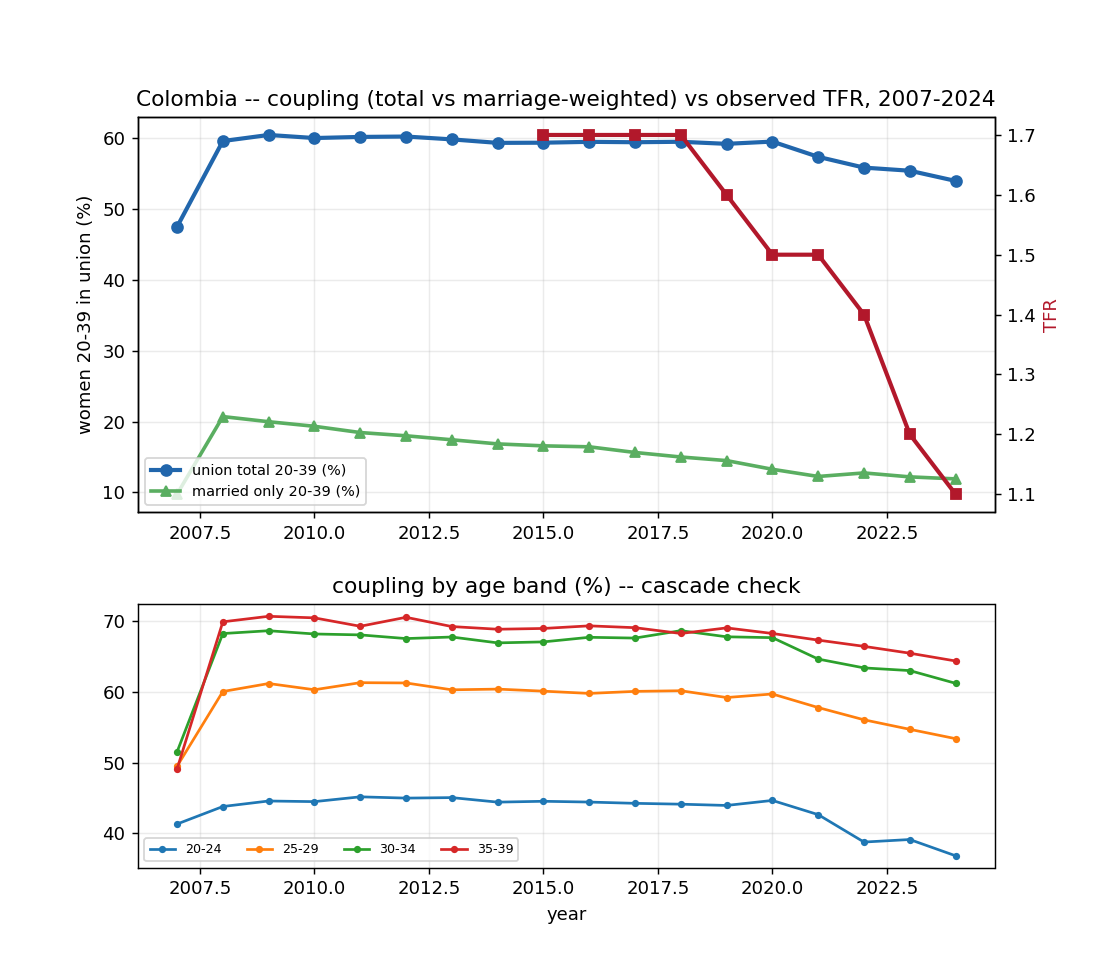
\includegraphics[width=\textwidth]{fig_coupling_vs_tfr_COL.png}
  \caption{Colombia (GEIH microdata, 2007--2024)}
\end{subfigure}
\hfill
\begin{subfigure}[b]{0.48\textwidth}
  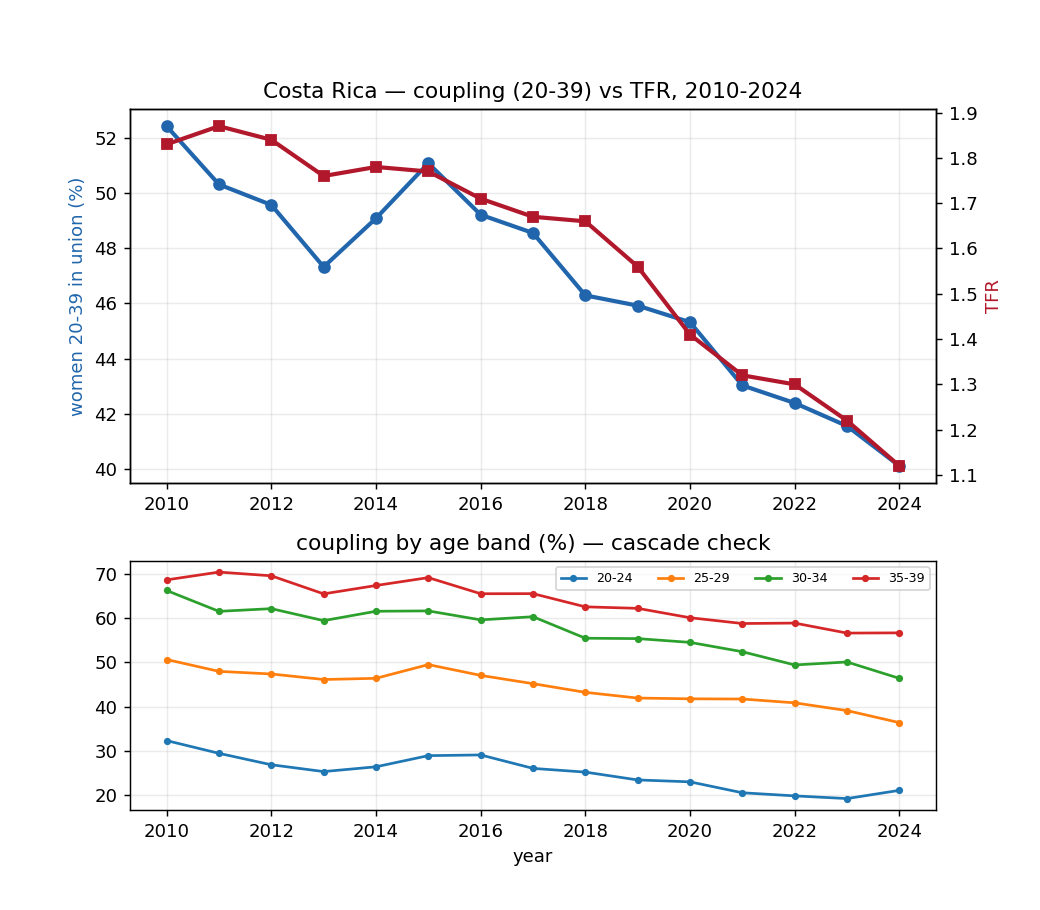
\includegraphics[width=\textwidth]{fig_coupling_vs_tfr_CRI.png}
  \caption{Costa Rica (ENAHO/REDATAM, 2010--2024)}
\end{subfigure}
\caption{Union composition of women 20--39 (married vs.\ cohabiting) against the
national TFR (comparison overlay only). Marriage collapses on a roughly flat
total-union base; cohabitation substitutes.}
\label{fig:coupling}
\end{figure}

\subsection{Data limitations: measurement}
\label{sec:datalim-measurement}

We flag the measurement limits here rather than in footnotes.
(i)~\emph{Colombia 2007.} The earliest GEIH year is a documented
frame/questionnaire outlier (total union 47.5 percent versus the 2008--2020
plateau near 59--60); all Colombian analysis treats 2008 as the first usable
composition year. (ii)~\emph{Argentina.} No official period TGF exists after
2021; our reconstruction is INDEC-anchored and labeled throughout. The
much-discussed INDEC credibility break of 2007--15 does \emph{not} contaminate
fertility: vital statistics are produced by DEIS, a separate institution.
(iii)~\emph{Chile.} The official TGF series has a 2010--21 publication gap,
filled here by births-implied TFR anchored to registry years.
(iv)~\emph{Pandemic-era collection.} Colombian household-survey collection in
2020--21 switched modes; we flag 2019--22 composition readings as potentially
affected and return to this in Sections~\ref{sec:model}
and~\ref{sec:limitations}. (v)~\emph{Tempo.} Registry TFRs are period measures;
where levels are anchored we also report a tempo-adjusted sensitivity in the
spirit of \citet{bongaarts1998} (a $+0.10$ TFR adjustment changes the Mexican
comparator's implied population by roughly 2 percent); none of the paper's
claims rests on the distinction.

% =============================================================================
% §3 Candidate mechanisms (M2) — three separable hypotheses; why smooth models
% struggle with fast collapse; the ABM as the device that separates predictions.
% =============================================================================
\section{Candidate Mechanisms and Their Signatures}
\label{sec:mechanisms}

Three families of mechanism could generate a marriage-composition collapse of
the observed speed. They are not mutually exclusive, but they carry different
observable signatures, which is what makes discrimination possible.

\paragraph{H$_{\text{cohort}}$: cohort replacement.}
Successive birth cohorts enter adulthood with durably lower marriage propensity
--- formed by education expansion, structural change, and the ideational change
of the Second Demographic Transition \citep{callesvogl2026} --- and the stock
composition shifts as these
cohorts flow through the age distribution. The signature: change localizes on
\emph{cohort} lines in an age--period--cohort decomposition; within a cohort,
behavior is comparatively stable; the aggregate can nonetheless accelerate
purely mechanically, as steep-gradient cohorts come to dominate the observed
age range.

\paragraph{H$_{\text{shock}}$: exogenous period shock.}
A calendar-time force common to all living cohorts --- an economic shock, a
policy change, a pandemic --- shifts marriage entry for everyone at once. The
signature: change localizes on \emph{period} lines, visible as parallel shifts
across cohorts at the same calendar date, with no dependence on the prevailing
composition itself.

\paragraph{H$_{\text{cascade}}$: within-cohort reflexive cascade.}
The mechanism behind most ``fast-dynamics'' narratives: individuals respond to
the behavior of their reference group, so that as non-marriage spreads, the
social cost of not marrying falls, generating self-reinforcing acceleration ---
a norm cascade or tipping dynamic. The signature is \emph{state dependence with
an amplifying sign}: within a cohort, marriage decline must be \emph{larger}
where the reference-group not-married share is already high. This is the only
mechanism of the three that is genuinely reflexive, and identifying it from
observational data confronts the classical reflection problem
\citep{manski1993}; Section~\ref{sec:discrimination} states how our design
addresses the sign-based, within-cohort version of the test.

Why not adjudicate with a standard smooth model? Because the phenomenon's
defining feature --- late acceleration --- is exactly what smooth aggregate
specifications absorb rather than explain. A logistic trend fitted to the
married share will always ``fit'' a collapse after the fact; it cannot say
whether the curvature came from cohort turnover, a dated shock, or feedback.
We therefore proceeded in two deliberately separated steps. First, the
econometric discrimination of Section~\ref{sec:discrimination}, which asks the
data directly which signature is present. Second, a generative test: we built
an agent-based implementation of the \emph{cascade} hypothesis --- a
coordination threshold in partnership formation, the formalization of the
tipping narrative --- and calibrated it to the composition data. That model was
a genuine, live candidate, not a straw man: with its threshold active it
generated a real, endogenous marriage decline, and removing the threshold
flipped the generated fertility path from collapse to increase (the mechanism
was doing the work). It nonetheless failed in a specific, diagnostic way: the
calibrated threshold produced a smooth glide --- roughly $-0.02$ per year in
generated TFR, about 55 percent of the observed magnitude --- with none of the
observed late acceleration, and its failure shaped the discrimination design
that follows. Cascade dynamics, when actually calibrated to composition data,
do not produce the observed shape; the question became which non-reflexive
structure does.

% =============================================================================
% §4 Discrimination — identification (M3 / R3). β>0 everywhere; COL cohort-
% dominant + small exogenous period; CRI cohort-leaning; 2c-i individual
% confirmation; explicit identification-strategy statement; ecological caveats.
% =============================================================================
\section{Discriminating the Mechanism: APC Curvature and the Sign of State
Dependence}
\label{sec:discrimination}

\subsection{Identification strategy, stated plainly}
\label{sec:idstrategy}

Two quantities identify the discrimination; both were fixed, with their decision
rule, before the estimates were run.

\emph{First, where the change localizes.} We build birth-year pseudo-cohorts
from the repeated cross-sections and decompose the married (and cohabiting)
share into age, period, and cohort components. Because the linear APC trends
are not separately identified, we rest nothing on them: only
\emph{curvature} (identified second differences) enters the verdict --- where
does the \emph{acceleration} sit, on cohort lines or on period lines? Age-band
fixed effects and within-band estimation keep Lexis artifacts out of the
curvature.

\emph{Second, the sign of state dependence.} For the cascade hypothesis the
decisive quantity is the coefficient $\beta$ on the \emph{lagged reference-group
not-married share} in a within-pseudo-cohort regression of the change in
marriage outcomes. An amplifying cascade requires $\beta < 0$ and significant:
decline must be faster where non-marriage is already prevalent. A positive
$\beta$ --- decline \emph{smaller} where the reference share is high --- is the
opposite of the cascade signature: stabilizing, mean-reverting dynamics. To
guard against mechanical correlation, the reference group is varied across
specifications: the adjacent \emph{younger} cohort (primary), the adjacent
\emph{older} cohort (clean of own-cohort reflection), the whole 20--39
population (robustness), and the cohort's own lag (comparator). The
pre-registered rule required an amplifying $\beta$ under the primary and at
least one clean specification, in \emph{both} countries, for
H$_{\text{cascade}}$ to stand.

\subsection{The verdict: stabilizing, not self-reinforcing}
\label{sec:verdict}

Table~\ref{tab:beta} reports the full $\beta$ matrix at lag one, where the
signal concentrates (lag-two estimates collapse toward zero).

\begin{table}[t]
\centering
\caption{State-dependence coefficient $\beta$ on the lagged reference
not-married share (lag 1). Amplifying cascade requires $\beta<0$.}
\label{tab:beta}
\begin{tabular}{lcc}
\toprule
Reference-group specification & $\beta$ Costa Rica & $\beta$ Colombia \\
\midrule
Adjacent younger cohort (primary) & $+0.17$ & $+1.33$ \\
Adjacent older cohort (clean)     & $+0.16$ & $+0.61$ \\
Population 20--39 (robustness)    & $+0.29$ & $+0.97$ \\
Own lag (comparator)              & $+0.36$ & $+0.98$ \\
\bottomrule
\end{tabular}
\end{table}

$\beta > 0$ in every specification, in both countries: \emph{the cascade
signature is absent}. Within-cohort marriage decline is \emph{smaller}, not
larger, where the reference not-married share is already high, and the
pre-registered H$_{\text{cascade}}$ condition fails comprehensively.
Descriptively the estimated dynamics are mean-reverting; we use
``stabilizing'' in that descriptive sense only, without attaching a
behavioral mechanism to the positive sign --- the design licenses the
rejection of the amplifying signature, not an interpretation of its opposite.

The localization completes the picture. In Colombia, curvature localizes on
\emph{cohort} lines (married-share curvature RMS 0.007 on period lines versus
0.014 on cohort lines), with a statistically unambiguous period component
(F-test $p \approx 3\times10^{-6}$) that is \emph{small} relative to the cohort
step-down --- and, crucially, non-reflexive: because $\beta$ is not amplifying,
that period component carries an \emph{exogenous-shock} signature, not
endogenous feedback. In Costa Rica the period effect is not statistically
present at all ($p = 0.18$), leaving a cohort-replacement reading. The
structure, in both countries, is
H$_{\text{cohort}}$ --- dominant cohort replacement --- with a secondary
H$_{\text{shock}}$ overlay in Colombia. Figure~\ref{fig:apc} shows the
pseudo-cohort lines and the identified curvature; Figure~\ref{fig:beta} the
$\beta$ estimates with confidence intervals by specification.

\begin{figure}[t]
\centering
\begin{subfigure}[b]{0.48\textwidth}
  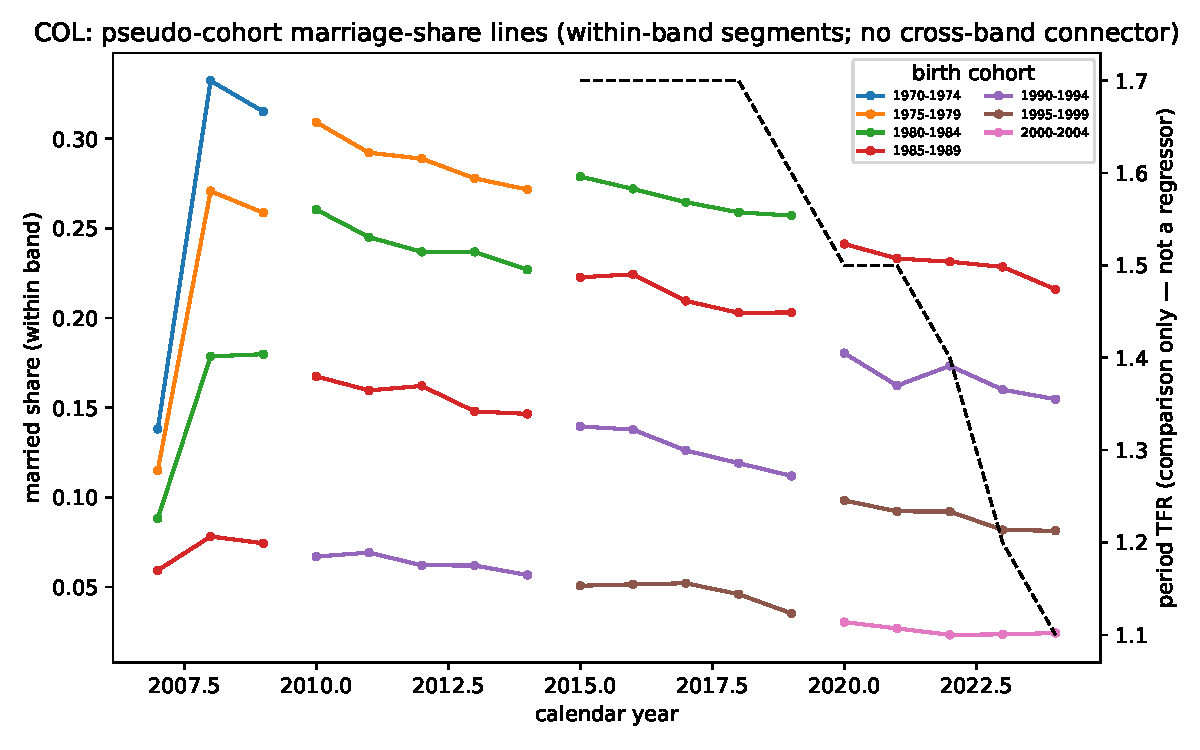
\includegraphics[width=\textwidth]{fig_cohortlines_COL.pdf}
  \caption{Colombia: pseudo-cohort lines}
\end{subfigure}
\hfill
\begin{subfigure}[b]{0.48\textwidth}
  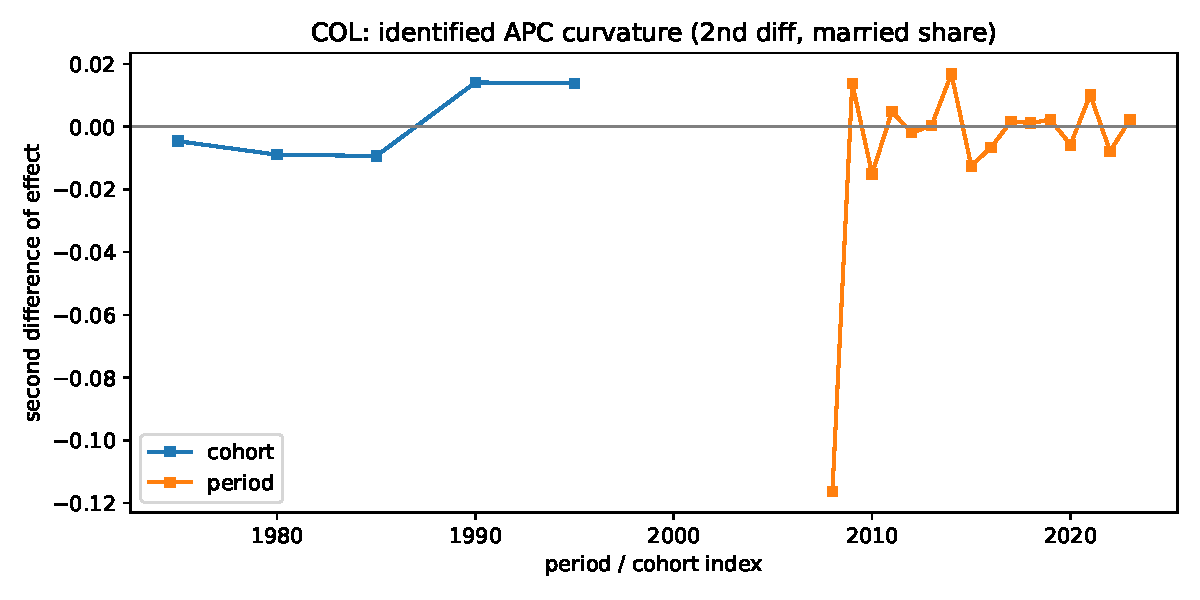
\includegraphics[width=\textwidth]{fig_apc_curvature_COL.pdf}
  \caption{Colombia: identified APC curvature}
\end{subfigure}
\caption{Localization of the change (Colombia; Costa Rica in the online
appendix). Acceleration sits on cohort lines; the period overlay is real but
small.}
\label{fig:apc}
\end{figure}

\begin{figure}[t]
\centering
\begin{subfigure}[b]{0.48\textwidth}
  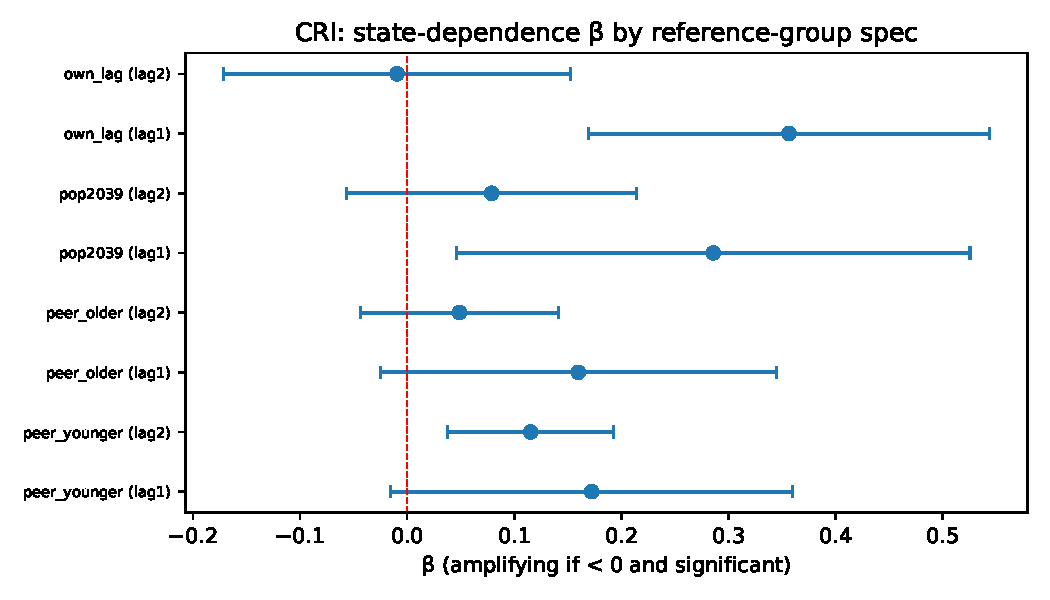
\includegraphics[width=\textwidth]{fig_beta_ci_CRI.pdf}
  \caption{Costa Rica}
\end{subfigure}
\hfill
\begin{subfigure}[b]{0.48\textwidth}
  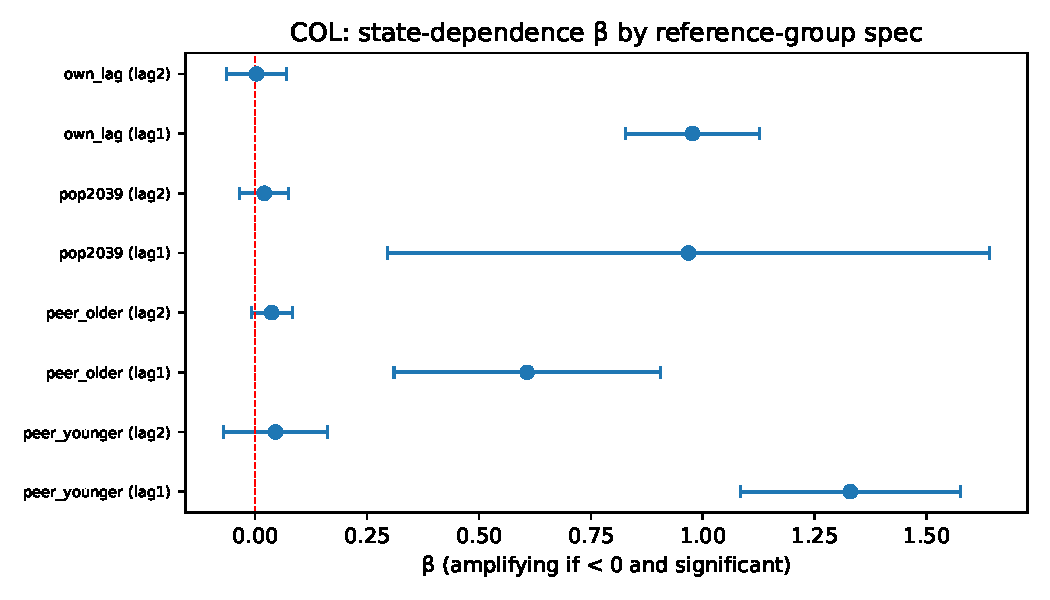
\includegraphics[width=\textwidth]{fig_beta_ci_COL.pdf}
  \caption{Colombia}
\end{subfigure}
\caption{State-dependence $\beta$ by reference-group specification, with
confidence intervals. Positive everywhere: stabilizing, not cascading.}
\label{fig:beta}
\end{figure}

\subsection{The individual-level confirmation}
\label{sec:individual}

The estimates above are cell-level: on repeated cross-sections, the
state-dependence test is a within-pseudo-cohort \emph{cell} regression, and an
ecological objection is available --- individual dynamics could differ from
cell dynamics. For Colombia, where person-level microdata permit it, we re-ran
the test at the individual-outcome level (a multinomial model of current union
status on the lagged reference share, person weights, within cohort--age
cells). The individual-level estimates confirm the cell-level verdict --- no
amplifying state dependence --- discharging the ecological objection for the
country where the period overlay made it most pointed. What repeated
cross-sections cannot deliver at any level is \emph{true individual
transitions}; that requires panel or event-history data (the Colombian ENDS
program), which we return to in Section~\ref{sec:limitations}.

Two caveats bound the verdict rather than undermine it. The 20--39 estimation
floor excludes the 15--19 entry margin --- a cascade igniting among teenagers
would be under-observed here; and both countries are high-cohabitation regimes,
so the non-cascade verdict does not automatically travel to marriage-dominant
systems (that is the out-of-sample prediction of
Section~\ref{sec:interpretation}, not an assumption).

% =============================================================================
% §5 Model & sufficiency (M4 / R4) — GLASS BOX per Fina §5/§A:
% reframe (4-parameter cohort microsimulation), equations in main text,
% algorithm box, calibration in the open, pre-registered gates, wall,
% κ–φ separability, ablations, non-fit convergences (fig2 signature),
% M3 residual, division of labor restated. ODD appendix cross-ref.
% =============================================================================
\section{A Transparent Sufficiency Test: Is Cohort Replacement Enough?}
\label{sec:model}

Section~\ref{sec:discrimination} identified the mechanism. This section asks a
different question, and it is important to keep the two separate: taking the
identified structure as given, is it \emph{sufficient}? Can cohort replacement
alone --- with no reflexivity anywhere --- generate the observed composition
collapse, its magnitude \emph{and} its late-loaded shape? The simulation model
below is never asked to identify anything; identification is econometric and
lives in Section~\ref{sec:discrimination}. The model's job is to test whether
the surviving mechanism quantitatively suffices, under an evaluation whose
success criteria were fixed before the model was run.

\subsection{The model is four interpretable parameters, not a black box}
\label{sec:modelspec}

The model is best described as a parsimonious cohort microsimulation. Beyond
five baseline demographic rates (calibrated, and interpretable as ordinary
formation/dissolution hazards), its entire mechanism content is \emph{four}
parameters: three describing how marriage propensity declines across birth
cohorts, and one describing how union formation tilts across birth cohorts.
There are no per-cohort free effects, no adaptive dynamics, no interaction
terms, and --- by construction --- no channel through which any agent's
transition depends on any other agent's state.

Each woman $i$ carries age $a_{it} \in \{15,\dots,49\}$, birth year $b_i$, and
union status $u_{it} \in \{\Sng, \Coh, \Mar\}$. One tick is one calendar year.
Annual transitions are:
\begin{align}
\Pr(\Sng \to \text{union})_{it} &= f_0 \,\phib[b_i],
  &&\text{of which married w.p. } m_0\,\kb[b_i], \text{ else cohabiting},
  \label{eq:formation}\\
\Pr(\Coh \to \Sng)_{it} &= \delta_c, \qquad
\Pr(\Coh \to \Mar \mid \text{no dissolution})_{it} = c_0 \,\kb[b_i],
  \label{eq:conversion}\\
\Pr(\Mar \to \Sng)_{it} &= \delta_m.
  \label{eq:dissolution}
\end{align}
In the cohabiting state, where dissolution and conversion compete, the two
risks are evaluated \emph{sequentially} --- dissolution first, then conversion
conditional on remaining in union, exactly as in Algorithm~\ref{alg:abm} ---
so the realized annual conversion probability is
$(1-\delta_c)\,c_0\,\kb$. This matches the reference implementation; the
conversion parameter $c_0$ is interpreted conditionally throughout.
The two cohort terms are
\begin{align}
\kb &= \kappa_\infty + \frac{1-\kappa_\infty}{1+\exp\{s\,(b-b_0)\}},
  \label{eq:kappa}\\
\phib &= \exp\{-\tau\,(b-1985)\}, \quad \text{clamped to } [0.2,\,3].
  \label{eq:phi}
\end{align}
Equation~\eqref{eq:kappa} is the paper's mechanism: a logistic decline in
cohort marriage propensity with exactly three parameters --- a floor
$\kappa_\infty$ (the marriage propensity of the newest cohorts relative to the
oldest), a midpoint $b_0$ (the birth cohort at which the decline is halfway),
and a slope $s$ (how compressed the across-cohort change is). It multiplies
both marriage-entry margins --- the formation split in~\eqref{eq:formation} and
the conversion hazard in~\eqref{eq:conversion} --- and nothing else.
Equation~\eqref{eq:phi} is a one-parameter log-linear tilt in overall union
formation across cohorts. Old cohorts ($b \ll b_0$) have $\kb \approx 1$: the
baseline rates $\{f_0, m_0, c_0, \delta_c, \delta_m\}$ are simply the behavior
of pre-decline cohorts.

In a robustness specification we add an exogenous period shifter
$\pit = 1 - d\,/\,(1+\exp\{-s_p (t - t_p)\})$ multiplying the same
marriage-entry margins --- calendar time only, common to all cohorts, never a
function of prevailing composition (the Colombian period overlay of
Section~\ref{sec:discrimination}). As shown below, the data render it
dispensable, and the headline specification omits it entirely.

Algorithm~\ref{alg:abm} states the per-year update completely; the ODD protocol
appendix (Appendix~\ref{app:odd}) documents the model to the community
transparency standard \citep{grimm2020odd}, sufficient for reimplementation.

\begin{algorithm}[t]
\caption{One simulated year (population of $N$ women; one tick = one year)}
\label{alg:abm}
\begin{algorithmic}[1]
\For{each woman $i$ (order immaterial; no interaction)}
  \State $\kappa \gets \kb[b_i]$;\quad $\varphi \gets \phib[b_i]$
    \Comment{depends only on own birth year}
  \If{$u_i = \Sng$}
    \State with prob.\ $f_0\varphi$: form union; married w.p.\
      $m_0\kappa$, else cohabiting
  \ElsIf{$u_i = \Coh$}
    \State with prob.\ $\delta_c$: $u_i \gets \Sng$; else with prob.\
      $c_0\kappa$: $u_i \gets \Mar$
  \Else
    \State with prob.\ $\delta_m$: $u_i \gets \Sng$
  \EndIf
  \State $a_i \gets a_i + 1$
  \If{$a_i > 49$} \State replace: $a_i \gets 15$, $u_i \gets \Sng$,
    $b_i \gets t - 15$ \Comment{new entry cohort carries its own $\kb$}
  \EndIf
\EndFor
\State $t \gets t + 1$ \Comment{model step advances the calendar; nothing else}
\end{algorithmic}
\end{algorithm}

The no-reflexivity claim is verifiable in the code, not just the prose: the
agent update reads no other agent's state (no population shares, no
reference-group terms enter any transition), and the model-level step advances
the calendar only. Automated checks --- static source checks plus a runtime
registry of every data file opened during calibration --- are logged with the
repository (eleven checks per country, all passing).

\subsection{Calibration in the open}
\label{sec:calibration}

\emph{Targets.} The observed per-band (20--24 through 35--39) married and
cohabiting shares, all available years: Costa Rica ENAHO 2010--2024; Colombia
GEIH 2008--2024 (2008 seed per the documented 2007 frame outlier,
Section~\ref{sec:datalim-measurement}). The initial population is seeded at
the first observed year's composition.

\emph{Loss.} Composition only:
\begin{equation}
\mathcal{L} \;=\; \sum_{\text{bands}} \sum_{\text{years}}
\left[ \left(m^{\text{sim}} - m^{\text{obs}}\right)^2
     + \left(c^{\text{sim}} - c^{\text{obs}}\right)^2 \right].
\label{eq:loss}
\end{equation}

\emph{Identification wall.} The TFR never enters the loss, tunes no parameter,
and is not loaded during calibration (enforced by the runtime file registry).
Where a TFR path appears in this paper it is a comparison overlay only.

\emph{Free versus fixed.} Free, per country: the five baseline rates, the three
$\kb$ parameters, the $\phib$ tilt (and, in the robustness specification, the
three $\pit$ parameters). Fixed: the demographic scaffolding (age range,
seeding, closed-cohort replacement), reported in Appendix~\ref{app:odd}. The
resulting parameter-to-moment ratio is the most legible overfitting check:
\emph{nine} free parameters per country face 120 (Costa Rica: 4 bands
$\times$ 2 shares $\times$ 15 years) and 136 (Colombia: $4 \times 2 \times 17$)
target moments. Closed-cohort replacement holds cohort inflow constant ---
counterfactual under birth declines of 18--47 percent --- but the evaluation
metrics are computed on \emph{within-band composition shares}, which are
insulated from inflow scale by construction.

\emph{Optimizer.} Nelder--Mead in a boxed transform, four random restarts, 600
evaluations per country; inner evaluation ensembles of 12{,}000 agents
$\times$ 4 seeds; final reported ensembles of 50{,}000 agents $\times$ 16 seeds
(mean $\pm$ s.d.). The pipeline is deterministic given seeds; the Costa Rican
calibration, re-run end-to-end, reproduces its loss to all reported digits.

\emph{Pre-registered evaluation.} Three metrics were fixed, with their
thresholds, before the full calibration ran. On the equal-band-mean married
share: \textbf{M1}, magnitude capture --- the simulated share of the observed
seed-to-2024 fall --- must be at least $0.85$; \textbf{M2}, the late-window
share of the total decline (2017--2024 relative to the full window) must match
the observed within $\pm 0.10$; \textbf{M3}, the sign of the mean second
difference over 2015--2024 must match (does the decline accelerate or
decelerate late?).

\subsection{Results: sufficiency on magnitude and late-loading}
\label{sec:results}

\begin{table}[t]
\centering
\caption{Pre-registered sufficiency metrics, headline (cohort-only)
specification. Final ensembles, 50{,}000 agents $\times$ 16 seeds.}
\label{tab:gates}
\begin{tabular}{lccl}
\toprule
Metric (married, 20--39 equal-band) & Costa Rica & Colombia & Criterion \\
\midrule
M1 magnitude capture & 0.954 & 0.999 & $\geq 0.85$: \textbf{pass, pass} \\
M2 late-share, sim vs.\ obs & 0.490 / 0.581 & 0.468 / 0.459 & $|\Delta|\leq0.10$: \textbf{pass, pass} \\
M3 late-window $\Delta^2$ sign & $+$ / $+$ & $+$ / $-$ & same sign: pass, \textbf{fail} \\
\midrule
Composition loss~\eqref{eq:loss} & 0.0372 & 0.0246 &
  (threshold model: 0.0855) \\
\bottomrule
\end{tabular}
\end{table}

Table~\ref{tab:gates} reports the gates; Figure~\ref{fig:abmbands} the fit.
The verdict, stated precisely: \emph{sufficiency on magnitude and late-loading,
with one unreproduced shape residual.} The cohort-only model captures 95.4
(Costa Rica) and 99.9 (Colombia) percent of the observed married-share fall and
matches the late-loading of the decline within 0.09 and 0.01 respectively. The
residual is Colombia's M3: the observed series steepens slightly in the late
window (a 2019--22 kink in which both married and cohabiting shares break
trend) while the simulated path does not. Both second differences are near
zero; the kink coincides with pandemic-era survey collection
(Section~\ref{sec:datalim-measurement}) and/or a discrete shock, and its
resolution requires transition-level data
(Section~\ref{sec:limitations}). The miss is structural, not incidental: both
cohort terms are monotone in birth cohort --- $\phib$ in particular cannot
produce Colombia's flat-then-declining total-union path --- so the same
parsimony that disciplines the model is what surfaces here as the residual. A kink that a smooth model misses is not
evidence of a cascade; Section~\ref{sec:discrimination} tested for that
signature directly and rejected it. Honest margins: under the headline
specification Costa Rica's M2 sits nearer its tolerance than with the period
term included ($\Delta$ 0.091 versus 0.038), and the (ungated) cohabitation
magnitude capture drops to 0.63.

\begin{figure}[t]
\centering
\begin{subfigure}[b]{\textwidth}
  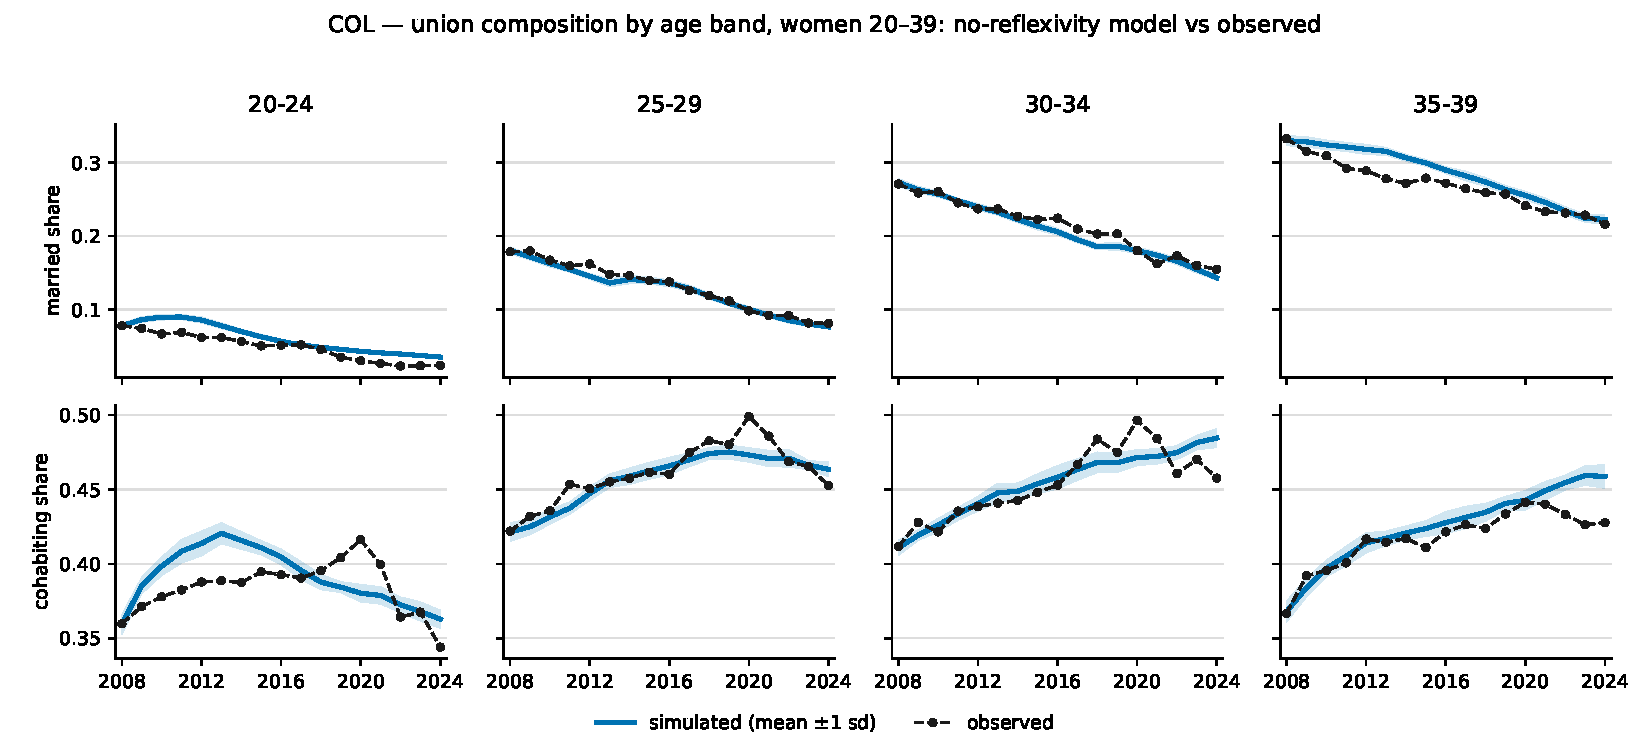
\includegraphics[width=\textwidth]{fig_abm_bands_COL.pdf}
  \caption{Colombia (seed 2008)}
\end{subfigure}\\[0.6em]
\begin{subfigure}[b]{\textwidth}
  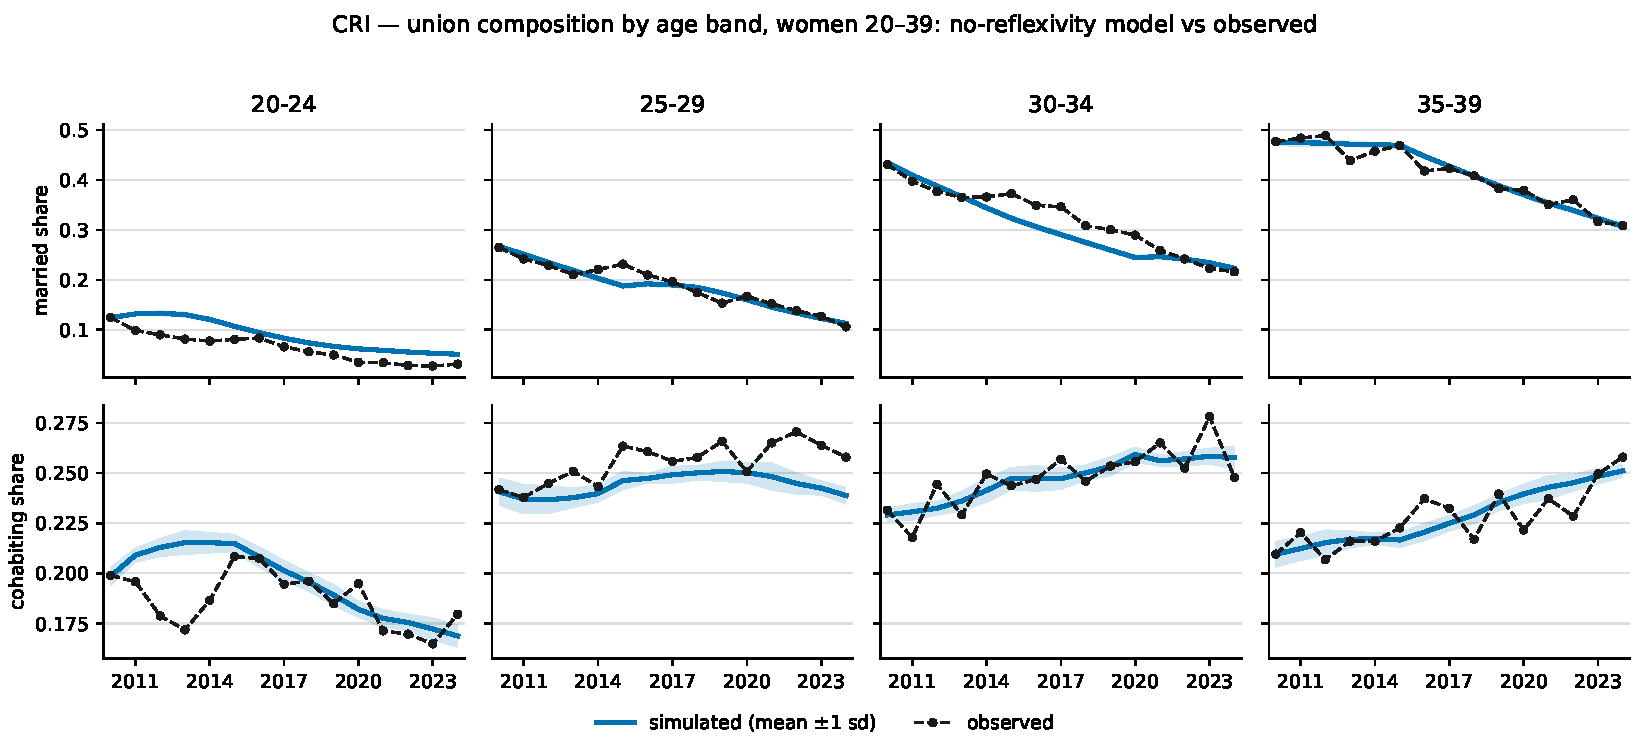
\includegraphics[width=\textwidth]{fig_abm_bands_CRI.pdf}
  \caption{Costa Rica (seed 2010)}
\end{subfigure}
\caption{Headline (cohort-only) model versus observed union composition, by
five-year age band: married (top rows) and cohabiting (bottom rows) shares,
simulated mean $\pm 1$ s.d.\ over 16 seeds against observed.}
\label{fig:abmbands}
\end{figure}

\subsection{Why the result is credible: what a black box could not do}
\label{sec:credibility}

Fit quality is table stakes --- a model handed a flexible mechanism should fit
a trajectory. The evidential weight lies in three properties a curve-fitting
box would not exhibit.

\paragraph{(i) A single recovered parameter matches an estimate the model never
saw.} The calibrated $\kb$ midpoints land at birth cohorts \textbf{1991.7}
(Costa Rica) and \textbf{1988.8} (Colombia). The APC decomposition of
Section~\ref{sec:discrimination} --- estimated by entirely different methods,
on cohort effects the simulation never touched --- places the married cohort
effects' sign crossover in the same 1985--1992 window
(Figure~\ref{fig:kappaapc}). Because $\kb$ is a three-parameter logistic, the
midpoint is one number, not a flexible profile that could have been bent to
agree: the convergence is non-circular. This is the paper's signature exhibit.

\begin{figure}[t]
\centering
\begin{subfigure}[b]{0.48\textwidth}
  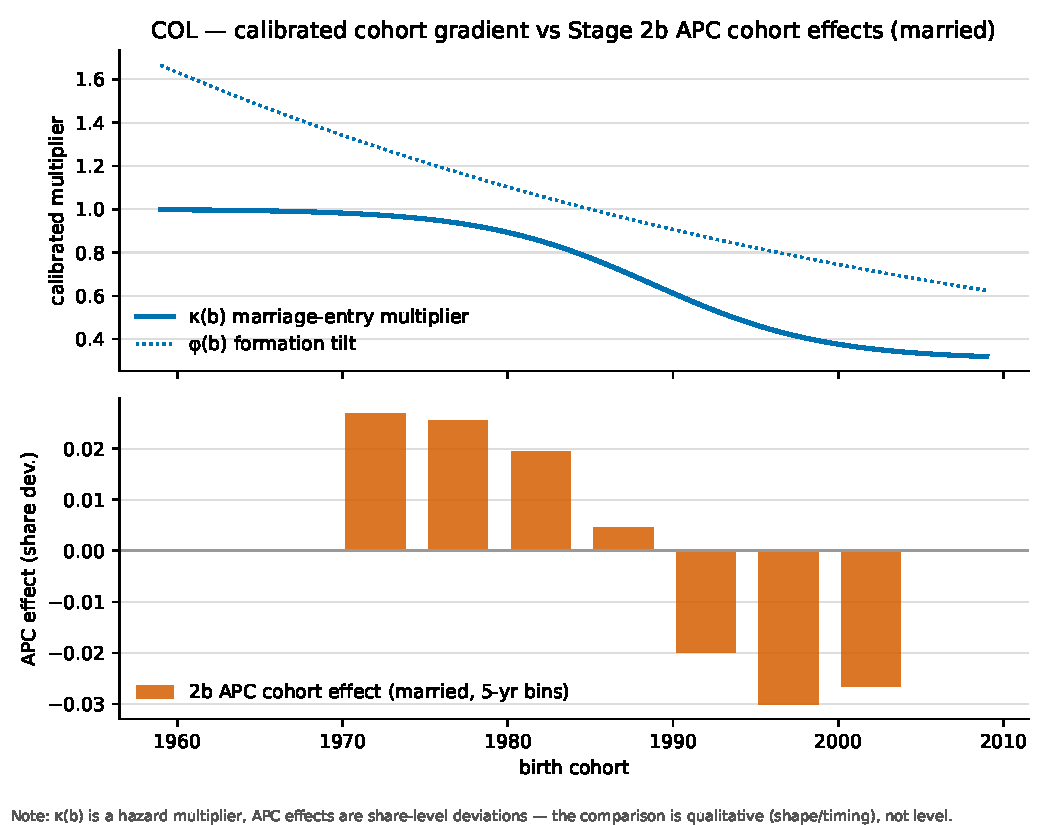
\includegraphics[width=\textwidth]{fig_kappa_apc_COL.pdf}
  \caption{Colombia}
\end{subfigure}
\hfill
\begin{subfigure}[b]{0.48\textwidth}
  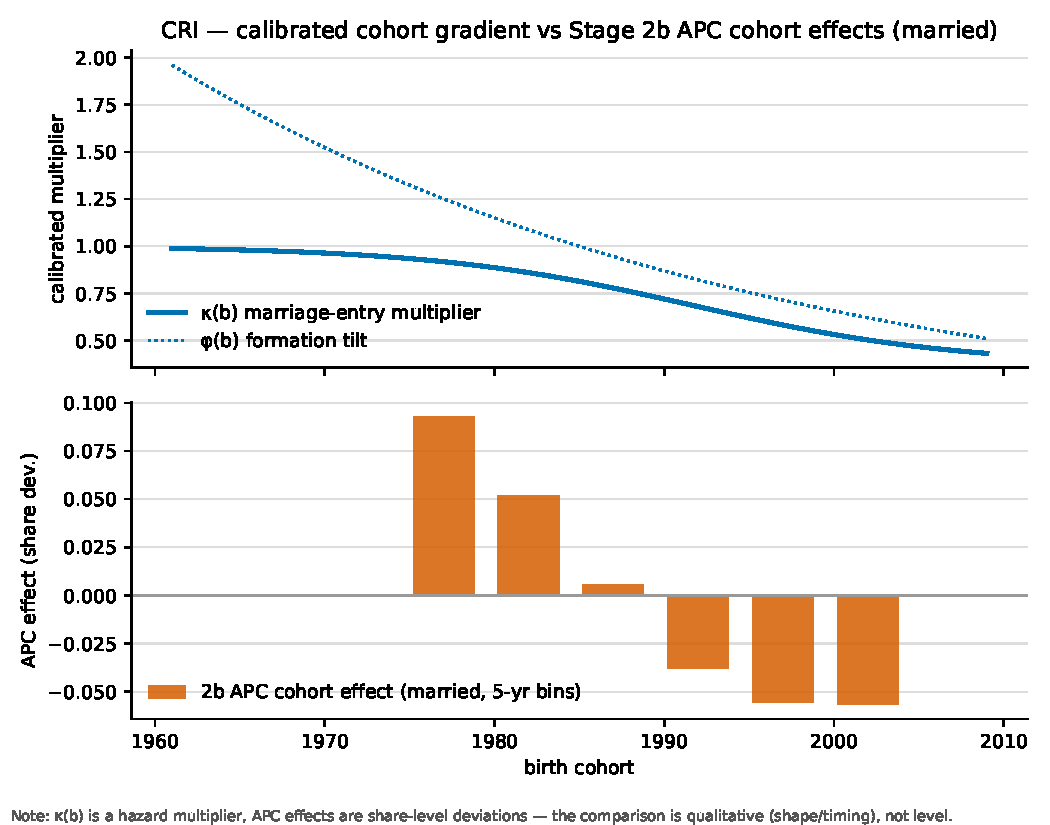
\includegraphics[width=\textwidth]{fig_kappa_apc_CRI.pdf}
  \caption{Costa Rica}
\end{subfigure}
\caption{The signature exhibit. Top panels: the calibrated cohort multiplier
$\kb$ (three parameters, calibrated to composition trajectories only). Bottom
panels: the independently estimated APC married cohort effects
(Section~\ref{sec:discrimination}). The calibrated midpoint recovers the APC
sign crossover the model was never fit to.}
\label{fig:kappaapc}
\end{figure}

\paragraph{(ii) Ablations reproduce the econometric decomposition.} Removing a
mechanism and \emph{fully recalibrating} the rest yields losses that mirror
Section~\ref{sec:discrimination}: without the cohort gradient, Colombia's loss
rises 63 percent (cohort replacement is essential exactly where the APC found
it dominant); without the period shifter, the loss is essentially unchanged in
both countries (Costa Rica $+6$ percent; Colombia slightly \emph{better}).
The apparent tension with Colombia's statistically significant period effect
dissolves on inspection: that effect is real but small (Section
\ref{sec:verdict}), and statistical existence is not quantitative necessity.
This is why the cohort-only model is the headline specification and the period
shifter a documented robustness term. A corollary worth stating against
ourselves: since a period-only model can also pass the magnitude gates,
band-level composition alone cannot discriminate the mechanisms --- which is
precisely why identification lives in Section~\ref{sec:discrimination} and the
model is asked only about sufficiency.

\paragraph{(iii) The mechanism's parameters are pinned by separate moments.}
Both cohort terms act on union behavior, so one may ask whether they are
separately identified or a disguised degree-of-freedom. They are separable by
construction: $\kb$ multiplies only marriage-\emph{entry} margins, both of
which leave union status unchanged (a formation splits into married or
cohabiting either way; a conversion moves within union), so $\kb$ is
union-total-neutral; $\phib$ multiplies formation itself and moves the union
total directly. Paired-seed perturbations at the calibrated parameters confirm
it: perturbing $\kappa_\infty$ moves the married share with the union total
essentially unchanged (response ratios 11.6 in Costa Rica, 102 in Colombia),
while perturbing $\tau$ does the reverse (ratios 0.32 and 0.05). The married
split pins $\kappa$; the union total pins $\varphi$.

Finally, the comparison that frames the exercise: this four-parameter,
no-feedback model fits the composition data \emph{better} than the calibrated
coordination-threshold model it replaced (losses 0.037/0.025 versus 0.086 on
the identical target) --- the reflexive mechanism was not removed at the cost
of fit, but with a gain.

A comparison-only overlay of the generated fertility path against the national
TFR appears in the online appendix figures; consistent with the identification
wall, we attach no claim to it --- its level rides a placeholder fertility
schedule, and the fertility-magnitude question requires union-specific
fertility rates that are the subject of ongoing data acquisition
(Section~\ref{sec:limitations}).

% =============================================================================
% §6 Interpretation (R5) — SDT channel-assisted compression; cohort-diffusion ↔
% cohort-dominance; Esteve anchor; ARG/CHL falsifiable prediction.
% Non-load-bearing: the paper stands on R1–R4.
% =============================================================================
\section{Interpretation: Channel-Assisted Compression of the Second
Demographic Transition}
\label{sec:interpretation}

The results so far stand on their own: a measured collapse
(Section~\ref{sec:phenomenon}), an identified structure
(Section~\ref{sec:discrimination}), and a sufficient parsimonious mechanism
(Section~\ref{sec:model}). This section offers the frame that makes them
cohere; the paper's claims do not depend on it.

The Second Demographic Transition describes ideational change ---
individualization, secularization, the decoupling of partnership from marriage
and of marriage from childbearing --- diffusing across cohorts
\citep{lesthaeghe1986twee, vandekaa1987, lesthaeghe2010}. Its standard account
explains direction well and tempo poorly: cohort-borne ideational change is
ordinarily a slow mechanism. What Latin America adds is a pre-existing
\emph{channel}. The region has maintained, since the colonial period, a dual
nuptiality system in which consensual union is a socially recognized,
institutionally familiar alternative to marriage --- massively expanded in the
recent ``cohabitation boom'' \citep{esteve2012}. Where that channel is already
wide, an arriving cohort that has absorbed SDT preferences does not need to
pioneer a new living arrangement, defy strong sanctions, or wait for
institutions to adapt; it flows into an existing one. The channel converts
ideational change into behavioral change at the speed of cohort succession
rather than the slower speed of institutional innovation --- \emph{compression},
assisted by the channel.

This reading knits the empirical pieces together. It explains why the change
localizes on cohort lines with stabilizing within-cohort dynamics
(Section~\ref{sec:discrimination}): the action is between cohorts, not within
them. It explains why a three-parameter cohort gradient suffices
(Section~\ref{sec:model}): the mechanism genuinely is a compressed
across-cohort shift in marriage propensity. And it explains the convergence of
our two independent lenses --- the econometric cohort \emph{dominance} and the
demographic account of cohort \emph{diffusion} are two faces of the same
object, and the model's recovered inflection at birth cohorts 1989--1992 dates
where the compression concentrated.

The frame also does what a frame should: it generates a falsifiable
out-of-sample prediction. If the consensual-union channel is the speed
mechanism, then in marriage-dominant regimes where the channel is narrow ---
Argentina and Chile are the natural regional cases, with the channel-relevant
composition series still under construction --- fertility decline of comparable
depth should be \emph{slower or differently structured}: less
marriage-to-cohabitation substitution at flat union totals, more decline within
existing union types, and weaker cohort localization. Both countries have
experienced deep declines (Section~\ref{sec:phenomenon}); the composition
anatomy of those declines is the test. We state the prediction now, before the
data are assembled, in the same pre-registration spirit as the rest of the
paper. Confirmation would establish the channel as the compression mechanism;
disconfirmation would bound the frame without touching the identified
cohort-replacement structure of Sections~\ref{sec:discrimination}
and~\ref{sec:model}.

% =============================================================================
% §7 Scope & limitations (M5) — inferential data-limitations subsection;
% claims-discipline constraints stated as scope conditions.
% =============================================================================
\section{Scope and Limitations}
\label{sec:limitations}

We state the paper's boundaries as claims we do \emph{not} make, each tied to
the data or design feature that enforces it.

\subsection{Data limitations: inference}
\label{sec:datalim-inference}

\paragraph{Pseudo-panels, not transitions.} All state-dependence estimates rest
on repeated cross-sections: within-pseudo-cohort cell dynamics, individual
\emph{outcomes} (Section~\ref{sec:individual}), but never observed individual
\emph{transitions}. First-union timing shifts can masquerade as composition
change in a pseudo-panel; the tempo margin is flagged, not resolved. And the
limitation should be stated at full strength: a no-reflexivity model sufficing
at the annual cell level does not \emph{close} the amplification question ---
it \emph{relocates} it. If a coordination dynamic operates anywhere, it would
live in first-union \emph{timing}, at sub-annual resolution, among the 15--19
entrants our estimation floor never observes --- scales at which annual
repeated cross-sections are blind by construction. The Colombian ENDS
event-history program is therefore not merely the resolution of the 2019--22
shape residual (Section~\ref{sec:results}); it is \emph{the test of sub-annual
amplification that the annual data cannot perform}. That is the honest content
of ``reflexivity not disproven.''

\paragraph{The 15--19 entry margin is unobserved.} The 20--39 estimation floor
excludes teenagers --- the plausible vanguard of any norm cascade. A cascade
igniting at 15--19 and arriving in our window already converted into cohort
heterogeneity would be under-observed. This is the one qualification we place
on the non-cascade verdict, and it is testable with entry-margin data.

\paragraph{Reflexivity: not warranted, not disproven.} Our design tests the
within-cohort, sign-based cascade signature, and the data reject it. We do not
claim to have disproven all reflexive mechanisms --- reflection-problem
identification limits are real \citep{manski1993} --- only that the mechanism's
observable signature is absent where it should appear, at both the cell and
individual-outcome level, in both countries. Transition-level data can reopen
the question; nothing else in this paper should.

\subsection{Scope conditions on the claims}

\paragraph{Composition, not fertility magnitude.} The sufficiency result of
Section~\ref{sec:model} concerns the \emph{union-composition} collapse. We make
no claim that the identified mechanism quantitatively accounts for the TFR
collapse: that requires union-specific fertility schedules (in particular the
cohabiting-to-married fertility differential), for which the required
married-specific rates are still under acquisition. The generated-TFR overlay
shown with the model is comparison-only by construction (the identification
wall of Section~\ref{sec:calibration}).

\paragraph{Two high-cohabitation regimes.} The identification and sufficiency
results cover Costa Rica and Colombia. External validity to marriage-dominant
regimes is precisely the out-of-sample prediction of
Section~\ref{sec:interpretation}, not an assumption --- Argentina and Chile are
the designated tests.

\paragraph{No tempo decomposition.} The model's fertility layer is
parity-independent and makes no tempo claim; where TFR levels are anchored, a
tempo-adjusted sensitivity in the spirit of \citet{bongaarts1998} is reported
alongside (Section~\ref{sec:datalim-measurement}).

\paragraph{Aggregation honesty.} The Colombian individual-level confirmation
covers outcomes, not transitions; Costa Rican estimates remain cell-level
(pre-tabulated REDATAM aggregates). We flag rather than smooth this asymmetry;
the verdict is sign-based and agrees across every level at which it can be
computed.

\paragraph{Interpretation is severable.} The channel-assisted-compression frame
(Section~\ref{sec:interpretation}) organizes the results and generates the
prediction; the measured collapse, the non-cascade verdict, and the sufficiency
result do not depend on it.

% =============================================================================
% §8 Conclusion — arc restated; ARG/CHL forward hook; light policy resonance;
% ENDS as the resolving next step.
% =============================================================================
\section{Conclusion}
\label{sec:conclusion}

Latin America's fertility collapse is among the fastest on record, and fast
phenomena attract fast-dynamics explanations. We took the leading one
seriously enough to build it: a coordination-threshold model of reflexive norm
cascade, calibrated to the union-composition data. The data rejected it twice
--- generatively (a glide where the observations accelerate) and
econometrically (state dependence with the stabilizing sign, in every
specification, in both countries, at cell and individual-outcome level). What
survived is almost embarrassingly simple: successive cohorts arrive with
durably lower marriage propensity, and the observed collapse is the stock
composition catching up with the flow --- a compressed Second Demographic
Transition running through a consensual-union channel that was already wide.
A cohort microsimulation whose entire mechanism is four interpretable
parameters reproduces the collapse's magnitude and late-loading, and its one
recovered inflection point independently matches the econometric cohort
crossover. The exciting mechanism failed; the boring one, tested to
pre-registered standards, suffices.

Three things follow. For measurement: the collapse is invisible in smoothed
international series, and analysis or policy built on them will date it late
and understate it --- national registries and microdata are not optional here.
For interpretation: composition is the state variable. Where marriage and
cohabitation carry different fertility, a marriage collapse at flat union
totals is a fertility event, and projections that model union formation
without its composition will miss the mechanism. For policy, stated at the
modest level the evidence supports: the driver is cohort replacement, not a
within-cohort contagion --- interventions premised on interrupting a cascade
target a mechanism the data do not exhibit, while the actual structure implies
persistence, because cohorts already formed carry their propensities forward.

Two tests will discipline what we have claimed. The Argentine and Chilean
composition series will test the channel prediction out of sample: if the
consensual-union channel is the compression mechanism, marriage-dominant
regimes should collapse differently. And event-history data (the Colombian
ENDS program) will observe the transitions that repeated cross-sections cannot
--- resolving the one unreproduced shape residual, testing the excluded 15--19
entry margin, and providing the only evidence that could legitimately reopen
the reflexivity question. We have registered the predictions; the data will
adjudicate.


\section*{Statements and Disclosures}
\noindent\textbf{Use of AI tools.} This paper was prepared using an AI-assisted
research workflow: large language models (Anthropic Claude) were used, under
the author's direction and review, for data acquisition scripting, statistical
and simulation code, figure production, and manuscript drafting, following
written build instructions and pre-registered evaluation criteria fixed before
results were computed. All data come from the cited official sources; the
analysis pipeline is deterministic given seeds and available for replication
(Appendix~\ref{app:odd}). The author reviewed and takes full responsibility
for the content, claims, and any errors.\\[0.4em]
\noindent\textbf{Data and code availability.} See Appendix~\ref{app:odd}.\\[0.4em]
\noindent\textbf{Conflicts of interest.} None declared.

\bibliographystyle{plainnat}
\bibliography{references}

\appendix
% =============================================================================
% Appendix A — ODD protocol (Grimm et al. 2020, second update).
% The anti-black-box deliverable: sufficient for reimplementation.
% =============================================================================
\section{ODD Protocol for the Cohort Microsimulation}
\label{app:odd}

This appendix documents the model of Section~\ref{sec:model} following the ODD
(Overview, Design concepts, Details) protocol, second update
\citep{grimm2020odd}. Together with Algorithm~\ref{alg:abm} and
equations~\eqref{eq:formation}--\eqref{eq:phi}, it is intended to be sufficient
for independent reimplementation. The reference implementation (Julia,
Agents.jl) with all figure data is available in the project repository.

\subsection{Purpose and patterns}

\emph{Purpose:} to test whether cohort-entry heterogeneity in marriage
propensity --- with no social feedback of any kind --- is \emph{sufficient} to
reproduce the observed union-composition collapse among women 20--39 in Costa
Rica (2010--2024) and Colombia (2008--2024). The model is evaluated against
three pre-registered patterns: (M1) the magnitude of the married-share fall;
(M2) its late-loading; (M3) the sign of its late-window curvature
(Section~\ref{sec:calibration}). It is explicitly \emph{not} used for
identification (done econometrically, Section~\ref{sec:discrimination}),
fertility-magnitude claims, or projection.

\subsection{Entities, state variables, and scales}

\emph{Entities:} women; no other agent types, no spatial units, no collectives.
\emph{State variables per woman:} age $a \in \{15,\dots,49\}$ (single years);
birth year $b$ (fixed at entry); union status
$u \in \{\Sng,\Coh,\Mar\}$; parity (bookkeeping for the comparison-only
fertility overlay; no behavioral role). Two fixed background attributes
(education level, urban/rural) are carried for descriptive seeding realism but
enter no transition rule in this specification.
\emph{Scales:} one tick = one calendar year; population 50{,}000 women
(reported ensembles); horizon = seed year to 2024 (14 ticks Costa Rica, 16
Colombia).

\subsection{Process overview and scheduling}

Each tick, every woman executes, in order: (1) union transition per
equations~\eqref{eq:formation}--\eqref{eq:dissolution}; (2) fertility-overlay
draw (comparison bookkeeping only); (3) ageing by one year, with closed-cohort
replacement --- a woman exceeding 49 is replaced by a new 15-year-old single
woman with birth year $t-15$, who therefore carries her own cohort's $\kb$ and
$\phib$. The model-level step advances the calendar year; it computes nothing
else. Agent processing order is immaterial because agents do not interact
(Design concepts). Composition observables are measured after each tick.

\subsection{Design concepts}

\emph{Basic principles.} Cohort replacement as the carrier of behavioral
change: transition probabilities depend on own birth cohort and own state only.
The two cohort functions $\kb$ (marriage entry) and $\phib$ (union formation)
encode the Second Demographic Transition's across-cohort gradient in reduced
form.
\emph{Emergence.} The aggregate composition trajectory --- including its late
acceleration --- emerges from the interaction of the cohort gradient with the
age-structured stock-flow dynamics: nothing in the rules accelerates; the
acceleration is compositional.
\emph{Adaptation, objectives, learning, prediction.} None. Agents do not
decide, optimize, learn, or forecast; transitions are exogenous hazards. This
is by design --- the model is a sufficiency probe for a mechanism, not a
behavioral theory.
\emph{Sensing and interaction.} \textbf{None, verifiably.} No agent's
transition depends on any other agent's state or on any population aggregate.
The absence is enforced by automated checks: static source checks (the agent
update contains no cross-agent read; feedback identifiers from the rejected
threshold model are absent) and a runtime registry proving that only the
composition target file is opened during calibration. Eleven checks per
country; all pass.
\emph{Stochasticity.} Bernoulli draws for all transitions; seeded generators;
the full pipeline is deterministic given seeds (the Costa Rican calibration
reproduces its loss to all reported digits on re-run).
\emph{Collectives.} None.
\emph{Observation.} Per-band (20--24, 25--29, 30--34, 35--39) married and
cohabiting shares each tick; ensemble mean $\pm$ s.d.\ over 16 seeds.

\subsection{Initialization}

The population is seeded at the first observed year (Costa Rica 2010, Colombia
2008 --- the 2007 Colombian survey year is a documented frame outlier,
Section~\ref{sec:datalim-measurement}): ages uniform 15--49; birth year $=$
seed year $-$ age; union status drawn from the observed band-specific
married/cohabiting shares, with age-graded extrapolation to the unobserved
15--19 and 40--49 tails (ramp below the 20--24 band; held at the 35--39 level,
respectively). Pre-seed cohorts receive $\kb$ and $\phib$ from the same
parametric functions --- the seeded stock embodies the gradient.

\subsection{Input data}

Calibration target (the only file read during calibration): observed annual
per-band married/cohabiting shares --- Costa Rica ENAHO via INEC REDATAM
tabulations; Colombia DANE GEIH person microdata, pooled annual files,
person-weighted. National TFR series are loaded only after calibration, for
the comparison overlay. Every series carries per-row source and methodology
flags in the repository.

\subsection{Submodels and calibrated parameters}

The complete submodels are
equations~\eqref{eq:formation}--\eqref{eq:phi}. Table~\ref{tab:params} reports
the calibrated headline (cohort-only) parameters; the robustness specification
adds the period shifter $\pit$ (three parameters), whose ablation costs are
reported in Section~\ref{sec:credibility}.

\begin{table}[h]
\centering
\caption{Calibrated parameters, headline (cohort-only) specification.}
\label{tab:params}
\small
\begin{tabular}{llcc}
\toprule
& Interpretation & Costa Rica & Colombia \\
\midrule
$f_0$ & base union-formation hazard (single, /yr) & 0.067 & 0.126 \\
$m_0$ & married share of new unions (oldest cohorts) & 0.308 & 0.147 \\
$c_0$ & cohabitation$\to$marriage hazard (oldest cohorts) & 0.042 & 0.025 \\
$\delta_c$ & cohabitation dissolution hazard & 0.062 & 0.067 \\
$\delta_m$ & marriage dissolution hazard & 0.019 & 0.023 \\
\midrule
$\kappa_\infty$ & marriage-propensity floor, newest cohorts & 0.371 & 0.306 \\
$b_0$ & cohort-decline midpoint (birth year) & 1991.7 & 1988.8 \\
$s$ & cohort-decline steepness (/birth-yr) & 0.129 & 0.194 \\
$\tau$ & formation tilt (/birth-yr) & 0.028 & 0.020 \\
\midrule
& composition loss~\eqref{eq:loss} & 0.0372 & 0.0246 \\
\bottomrule
\end{tabular}
\end{table}

\subsection{Data and code availability}

The reference implementation, calibration harness (including the
pre-registered gates and the automated no-feedback/no-TFR checks with their
logs), figure data for every exhibit, and the archived superseded runs are
maintained in the project repository and will be deposited with the
publication version. Figures regenerate from stored figure-data files without
re-simulation; the full calibration re-runs in minutes on a workstation and is
deterministic given seeds.


\end{document}
